\documentclass[12pt,table]{article}
\usepackage{sectsty}
\usepackage[utf8]{inputenc}
\usepackage[utf8]{inputenc}
\usepackage{multirow}
\usepackage{siunitx}
\sisetup{
  per-mode=fraction
}
\DeclareSIUnit\lbf{\text{lbf}}
\usepackage{graphicx}
\usepackage{amsmath}
\usepackage{amssymb}
\usepackage[version=4]{mhchem}
\usepackage{longtable,tabularx}
\usepackage{times}
\usepackage[format=hang,font={small,bf}]{caption}
\usepackage{url}
\usepackage{float}
\setlength\topmargin{0pt}
\addtolength\topmargin{-\headheight}
\addtolength\topmargin{-\headsep}
\setlength\oddsidemargin{0pt}
\setlength\textwidth{\paperwidth}
\addtolength\textwidth{-2in}
\setlength\textheight{\paperheight}
\addtolength\textheight{-2in}
\usepackage{layout}
\usepackage[T1]{fontenc}
\usepackage[framed,numbered]{matlab-prettifier}
\lstset{
	style = Matlab-editor,
	basicstyle=\mlttfamily\small,
}
\usepackage{placeins}
\usepackage{indentfirst}
\usepackage{setspace}
\usepackage{array}
%\usepackage[table,xcdraw]{xcolor}
\usepackage{booktabs}
\sectionfont{\fontsize{12}{14}\selectfont}
\subsectionfont{\fontsize{12}{14}\selectfont}
\usepackage{gensymb}
\usepackage{secdot}
\usepackage{caption}
\usepackage{subcaption}
\usepackage{float}
\newcolumntype{P}[1]{>{\centering\arraybackslash}p{#1}}

%%%%%%%%%%%%%%%%%%%%%%%%%%%%%%% tikz stuff! %%%%%%%%%%%%%%%%%%%%%%%%%%%%%%%%%%%%
\usepackage{tikz}

\newcommand{\AxisRotatorX}[1][rotate=0]{%
    \tikz [x=-0.15cm,y=0.25cm,line width=.2ex,-stealth,#1] \draw (0,0) arc (150:-150:1 and 1);%
}

\newcommand{\AxisRotatorY}[1][rotate=0]{%
    \tikz [x=0.25cm,y=0.15cm,line width=.2ex,-stealth,#1] \draw (0,0) arc (-20:260:1 and 1);%
}

\newcommand{\AxisRotatorZ}[1][rotate=0]{%
    \tikz [x=0.20cm,y=0.25cm,line width=.2ex,-stealth,#1] \draw (0,0) arc (-110:160:1 and 1);%
}

%%%%%%%%%%%%%%%%%%%%%%%%%%%%%% Main Document %%%%%%%%%%%%%%%%%%%%%%%%%%%%%%%%%%%

\setlength\parindent{0.5in}

\renewcommand{\refname}{\normalsize}

\linespread{1.0}
% \pagestyle{myheadings}

\begin{document}


\begin{titlepage}
\hspace{0pt}
\vfill
\centering\large{\textbf{Illinois Space Society IREC Avionics Team}}
\par
\centering\large{\textbf{TARS Control System State-Space Model}}
\par

\vfill

\centering\textbf{March 6, 2021}
\thispagestyle{empty}
\end{titlepage}


\setcounter{page}{1}


\section{INTRODUCTION}

This article serves as a means of documenting the progress made by the IREC Avionics team in the development of a state-space model describing the dynamcis of a sounding rocket that is to compete in the Spaceport America Cup (formerly IREC) rocketry competition. The article is the culmination of the team's understanding in state-space control methods at the time of writing. We have limited expertise in the subject matter as we are a student team, therefore, care should be taken when referencing any material from this article.


\section{PRELIMINARIES}

\subsection{Rocket Frame of Reference}

In order to maintain congruency with roll-pitch-yaw conventions commonly employed in aerospace dynamics, the following reference frame will be used to express the vehicle's motion. The origin of this frame shall be the center of mass (COM) of the vehicle, with the $\boldsymbol{x}$ axis aligned to the axis of the rocket.


\begin{center}
\begin{tikzpicture}[x=1cm, y=1cm, z=-0.5cm]
    % Draw axes, angular velocity arrows
    \draw [->] (0,0,0) -- (4,0,0) node [at end, right] {$\boldsymbol{z}$}
                                  node [near end] {\AxisRotatorX}
                                  node [near end, above=0.3cm] {$\omega_z$ (yaw)};
    \draw [->] (0,0,0) -- (0,4.5,0) node [at end, left] {$\boldsymbol{x}$}
                                    node [very near end] {\AxisRotatorY}
                                    node (omega_x) [near end, above=0.5cm, right=0.2cm] {$\omega_x$ (roll)};
    \draw [->] (0,0,0) -- (0,0,4) node [at end, left] {$\boldsymbol{y}$}
                                  node [near end] {\AxisRotatorZ}
                                  node [right=0.5cm] {$\omega_y$}
                                  node [below=0.5cm, right=0.15cm] {(pitch)};
    % Draw rocket
    \draw (-0.3,2,0) -- (-0.3,-2,0) -- (0.3,-2,0) -- (0.3,2,0); % rocket body
    \draw (-0.3,2,0) arc (180:151:2.5); % nosecone left
    \draw (0.3,2,0) arc (0:29:2.5); % nosecone right
    \draw (-0.3,-1.2,0) -- (-0.6,-1.4,0) -- (-0.6,-1.8,0) -- (-0.3,-2,0); % Left Fin
    \draw (0.3,-1.2,0) -- (0.6,-1.4,0) -- (0.6,-1.8,0) -- (0.3,-2,0); % Right Fin
\end{tikzpicture}
\end{center}

\subsection{Tait-Brian Angles (aka Euler Angles)}

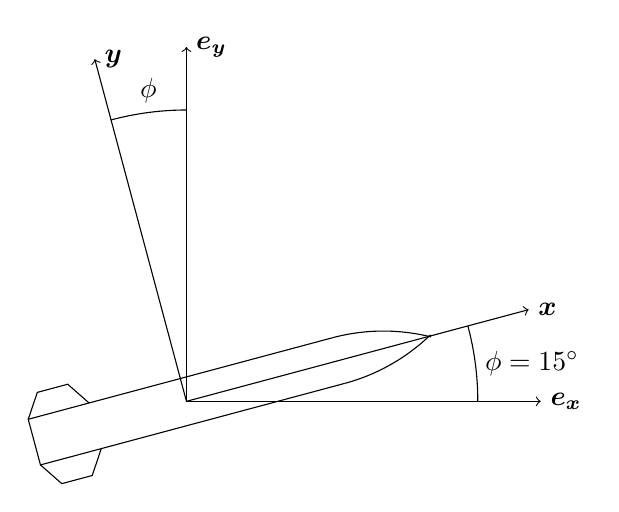
\begin{tikzpicture}[x=1cm, y=1cm]
    % Draw inertial frame
    \draw [->] (0,0) -- (4.5,0) node [at end, right] {$\boldsymbol{e_x}$};
    \draw [->] (0,0) -- (0,4.5) node [at end, right] {$\boldsymbol{e_y}$};
    % Draw rocket and rocket frame axes at 15 degree pitch
    \begin{scope} [rotate around z=-75]
      % Draw rocket frame axes x and y
      \draw [->] (0,0) -- (-4.5,0) node [at end, right] {$\boldsymbol{y}$};
      \draw [->] (0,0) -- (0,4.5) node [at end, right] {$\boldsymbol{x}$};
      % Draw Rocket
      \draw (-0.3,2,0) -- (-0.3,-2,0) -- (0.3,-2,0) -- (0.3,2,0); % rocket body
      \draw (-0.3,2,0) arc (180:151:2.5); % nosecone left
      \draw (0.3,2,0) arc (0:29:2.5); % nosecone right
      \draw (-0.3,-1.2,0) -- (-0.6,-1.4,0) -- (-0.6,-1.8,0) -- (-0.3,-2,0); % Left Fin
      \draw (0.3,-1.2,0) -- (0.6,-1.4,0) -- (0.6,-1.8,0) -- (0.3,-2,0); % Right Fin
    \end{scope}
    % Draw pitch angle arcs and labels
    \draw (3.7,0) arc (0:15:3.7) node [midway, right] {$\phi=15^{\circ}$};
    \draw (0,3.7) arc (90:105:3.7) node [midway, above] {$\phi$};
\end{tikzpicture}

\subsection{Quaternions}

\begin{equation*}
  q =
  \begin{bmatrix}
  q_0 \\ q_1 \\ q_2 \\ q_3
  \end{bmatrix},
  \quad
  \dot{q} =
  \begin{bmatrix}
  \dot{q_0} \\ \dot{q_1} \\ \dot{q_2} \\ \dot{q_3}
  \end{bmatrix}
\end{equation*}

Euler angle to quaternion conversion:

\begin{equation*}
  q(\phi, \theta, \psi) =
  \renewcommand\arraystretch{1.5}
  \begin{bmatrix}
  q_0 = \cos(\phi/2)\cos(\theta/2)\cos(\psi/2) + \sin(\phi/2)\sin(\theta/2)\sin(\psi/2) \\
  q_1 = \sin(\phi/2)\cos(\theta/2)\cos(\psi/2) - \cos(\phi/2)\sin(\theta/2)\sin(\psi/2) \\
  q_2 = \cos(\phi/2)\sin(\theta/2)\cos(\psi/2) + \sin(\phi/2)\cos(\theta/2)\sin(\psi/2) \\
  q_3 = \cos(\phi/2)\cos(\theta/2)\sin(\psi/2) - \sin(\phi/2)\sin(\theta/2)\cos(\psi/2) \\
  \end{bmatrix}
\end{equation*}

Quaternion to euler angle conversion:

\begin{equation*}
  \begin{bmatrix}
  \phi \\ \theta \\ \psi
  \end{bmatrix}
  =
  \renewcommand\arraystretch{1.5}
  \begin{bmatrix}
  \arctan(\frac{2(q_0q_1 + q_2q_3)}{1 - 2(q_1^2 + q_2^2)}) \\
  \arcsin(2(q_0q_2 - q_3q_1)) \\
  \arctan(\frac{2(q_0q_3 + q_1q_2)}{1 - 2(q_2^2 + q_3^2)}) \\
  \end{bmatrix}
\end{equation*}

\begin{equation*}
  \dot{q} = \frac{1}{2} \vec{\omega} \cdot q =
  \frac{1}{2}
  \begin{bmatrix}
  0 \\ \omega_x \\ \omega_y \\ \omega_z
  \end{bmatrix}
  \begin{bmatrix}
  q_0 \\ q_1 \\ q_2 \\ q_3
  \end{bmatrix} =
  \frac{1}{2}
  \begin{bmatrix}
  -q_1  & -q_2  & -q_3 \\
   q_0  & -q_3  &  q_2 \\
   q_3  &  q_0  & -q_1 \\
  -q_2  &  q_1  & q_0
  \end{bmatrix}
  \begin{bmatrix}
  \omega_x \\ \omega_y \\ \omega_z
  \end{bmatrix}
\end{equation*}


\end{document}
